\documentclass{beamer}
\usetheme{Pittsburgh}
\usepackage{xcolor}
\definecolor{USUBlue}{RGB}{26,57,89}
\usecolortheme[named=USUBlue]{structure}
\setbeamercolor{normal text}{fg=USUBlue}
\usepackage[utf8]{inputenc}
\usepackage{mathptmx}
\usepackage{tgbonum}
\usepackage{amssymb}
\usepackage{graphicx}
\usepackage{marvosym}
\usepackage[absolute, overlay]{textpos}
\usepackage{hyperref}
\usepackage{url}
\usefonttheme{structuresmallcapsserif}
\usefonttheme{serif}
\setbeamercolor{author}{fg=USUBlue}
\setbeamerfont{author}{size=\small}
\setbeamerfont{frametitle}{size=\large}
\setbeamertemplate{enumerate items}[default]
\author{Elita Baldridge, Department of Biology and the Ecology Center, Utah State University, Logan, UT, USA, @elitabaldridge\\Ethan White, Department of Wildlife Ecology \& Conservation and the Informatics Institute, University of Florida, Gainesville, FL, USA}
\title[17pt]{Ecologist in silico: Facilitating access for chronically ill/disabled ecologists}
\date{}
\setbeamertemplate{navigation symbols}{}

\usepackage[orientation=landscape,size=a0,scale=1.4,debug]{beamerposter}
 
\begin{document}
\begin{center} 
\begin{huge}
\rule{\linewidth}{0.25cm}
\textsc{%textsc makes text small caps
\\Ecologist in silico: Facilitating access for chronically ill/disabled ecologists\\
 }
\end{huge}  
\begin{large}
\textsc{Elita Baldridge}, Department of Biology and the Ecology Center, Utah State University, Logan, UT, USA, @elitabaldridge\\  
\textsc{Ethan White}, Department of Wildlife Ecology \& Conservation and the Informatics Institute, University of Florida, Gainesville, FL, USA, @ethanwhite\\
\end{large}
\end{center}
\begin{center}
\rule{\linewidth}{0.3cm}
\begin{minipage}{0.25\linewidth}
\begin{Large}
\vspace{0.5cm}
~\\
~\\
\textsc{Background}\\
\end{Large}
Members of under-represented groups face unconscious and conscious biases which create societal barriers to doing science.  Chronically ill/disabled scientists in particular often face physical as well as societal barriers.\\ 

\textsc{Disabilities can be visible or invisible, mental or physical, present with constant severity, get worse over time, or fluctuate from bad to less bad.\\ } 

I present recommendations to encourage ecology to become a more accessible discipline to those with chronic illness/disability, from a general perspective and on the scale of individual collaborations.\\

\begin{Large}
\textsc{The Default}
\begin{center}
\textsc{Inaccessibility.}\\
~\\
\end{center}
\end{Large}
\begin{Large}
\textsc{The Minimum}\\
\end{Large}
Provide accessibility information \textsc{without} request.\\
\begin{center}
\includegraphics[scale=1]{../sad-comparison/sad-data/dissertation/trinket-access-generator.png}\\
\textsc{Accessibility Statement Generator}
\end{center}
\begin{minipage}{0.3\textwidth}
\begin{small}
\includegraphics[scale=1]{../Pictures/Graphics/Access_generator.png} 
\end{small}
\end{minipage}
\begin{minipage}{0.67\textwidth}
\begin{small}
\url{https://goo.gl/7TjaF9}\\
\url{https://github.com/embaldridge/accessibility-statement-generator}\\
\end{small}
\end{minipage}
~\\
~\\
What accessibility accommodations are \textsc{and} are not available?  Making accessibility part of the planning lets disabled colleagues know that their presence is not an afterthought, and it saves a lot of time and heartache trying (and often failing) to get accommodations after the fact.\\
\end{minipage}
\hspace{1cm}
\begin{minipage}{0.42\linewidth}
\vspace{0.5cm}
\begin{center}
\begin{huge}
\textsc{Increasing Accessibility\\}
\end{huge}
\end{center}
~\\
~\\
\begin{Large}
\textsc{Conferences/Workshops\\}
\end{Large}
Mobility accessibility- provide signs, maps, reduce conference sprawl.\\
Consider making remote access available.\\
Have sign-language interpreters.\\
Provide trained sighted guides.\\
Consider special dietary requirements.\\
Try to confine events/activities from between 8 am to 5 pm.\\

\begin{Large}
\textsc{Talks\\}
\end{Large}
Livestream or record talk\\
Close caption video of talk\\
Consider color-blindness in slide design.\\
Provide handouts of slides, transcripts (both large and small format).\\
Verbally describe graphs and illustrations.\\

\begin{Large}
\textsc{Education\\}
\end{Large}
Set up accommodations to not require disclosure of condition from students.\\
Make available accommodations part of syllabus.\\
Assume students are telling the truth.\\
Record/livestream lectures.
Plan alternate lab exercises for students who need accommodation.
Provide handouts for lectures in advance.\\

\begin{Large}
\textsc{Research\\}
\end{Large}
Many people with disabilities can do field/lab work with proper accommodations.\\
Computational ecology, theory, and macroecological approaches are possible for those who can't do field work or other kinds of lab work.\\
Allow for remote working/flexible work schedule.\\
Use tools like GitHub to make remote work easier.\\
Open science facilitates research for unaffiliated researchers.\\
~\\
~\\
\begin{minipage}{0.60\linewidth}
Pdf of poster available here:\\
\url{https://github.com/embaldridge/posters-pres/blob/master/ESA_2015.pdf}\\
\end{minipage}
\hspace{2cm}
\begin{minipage}{0.3\linewidth}
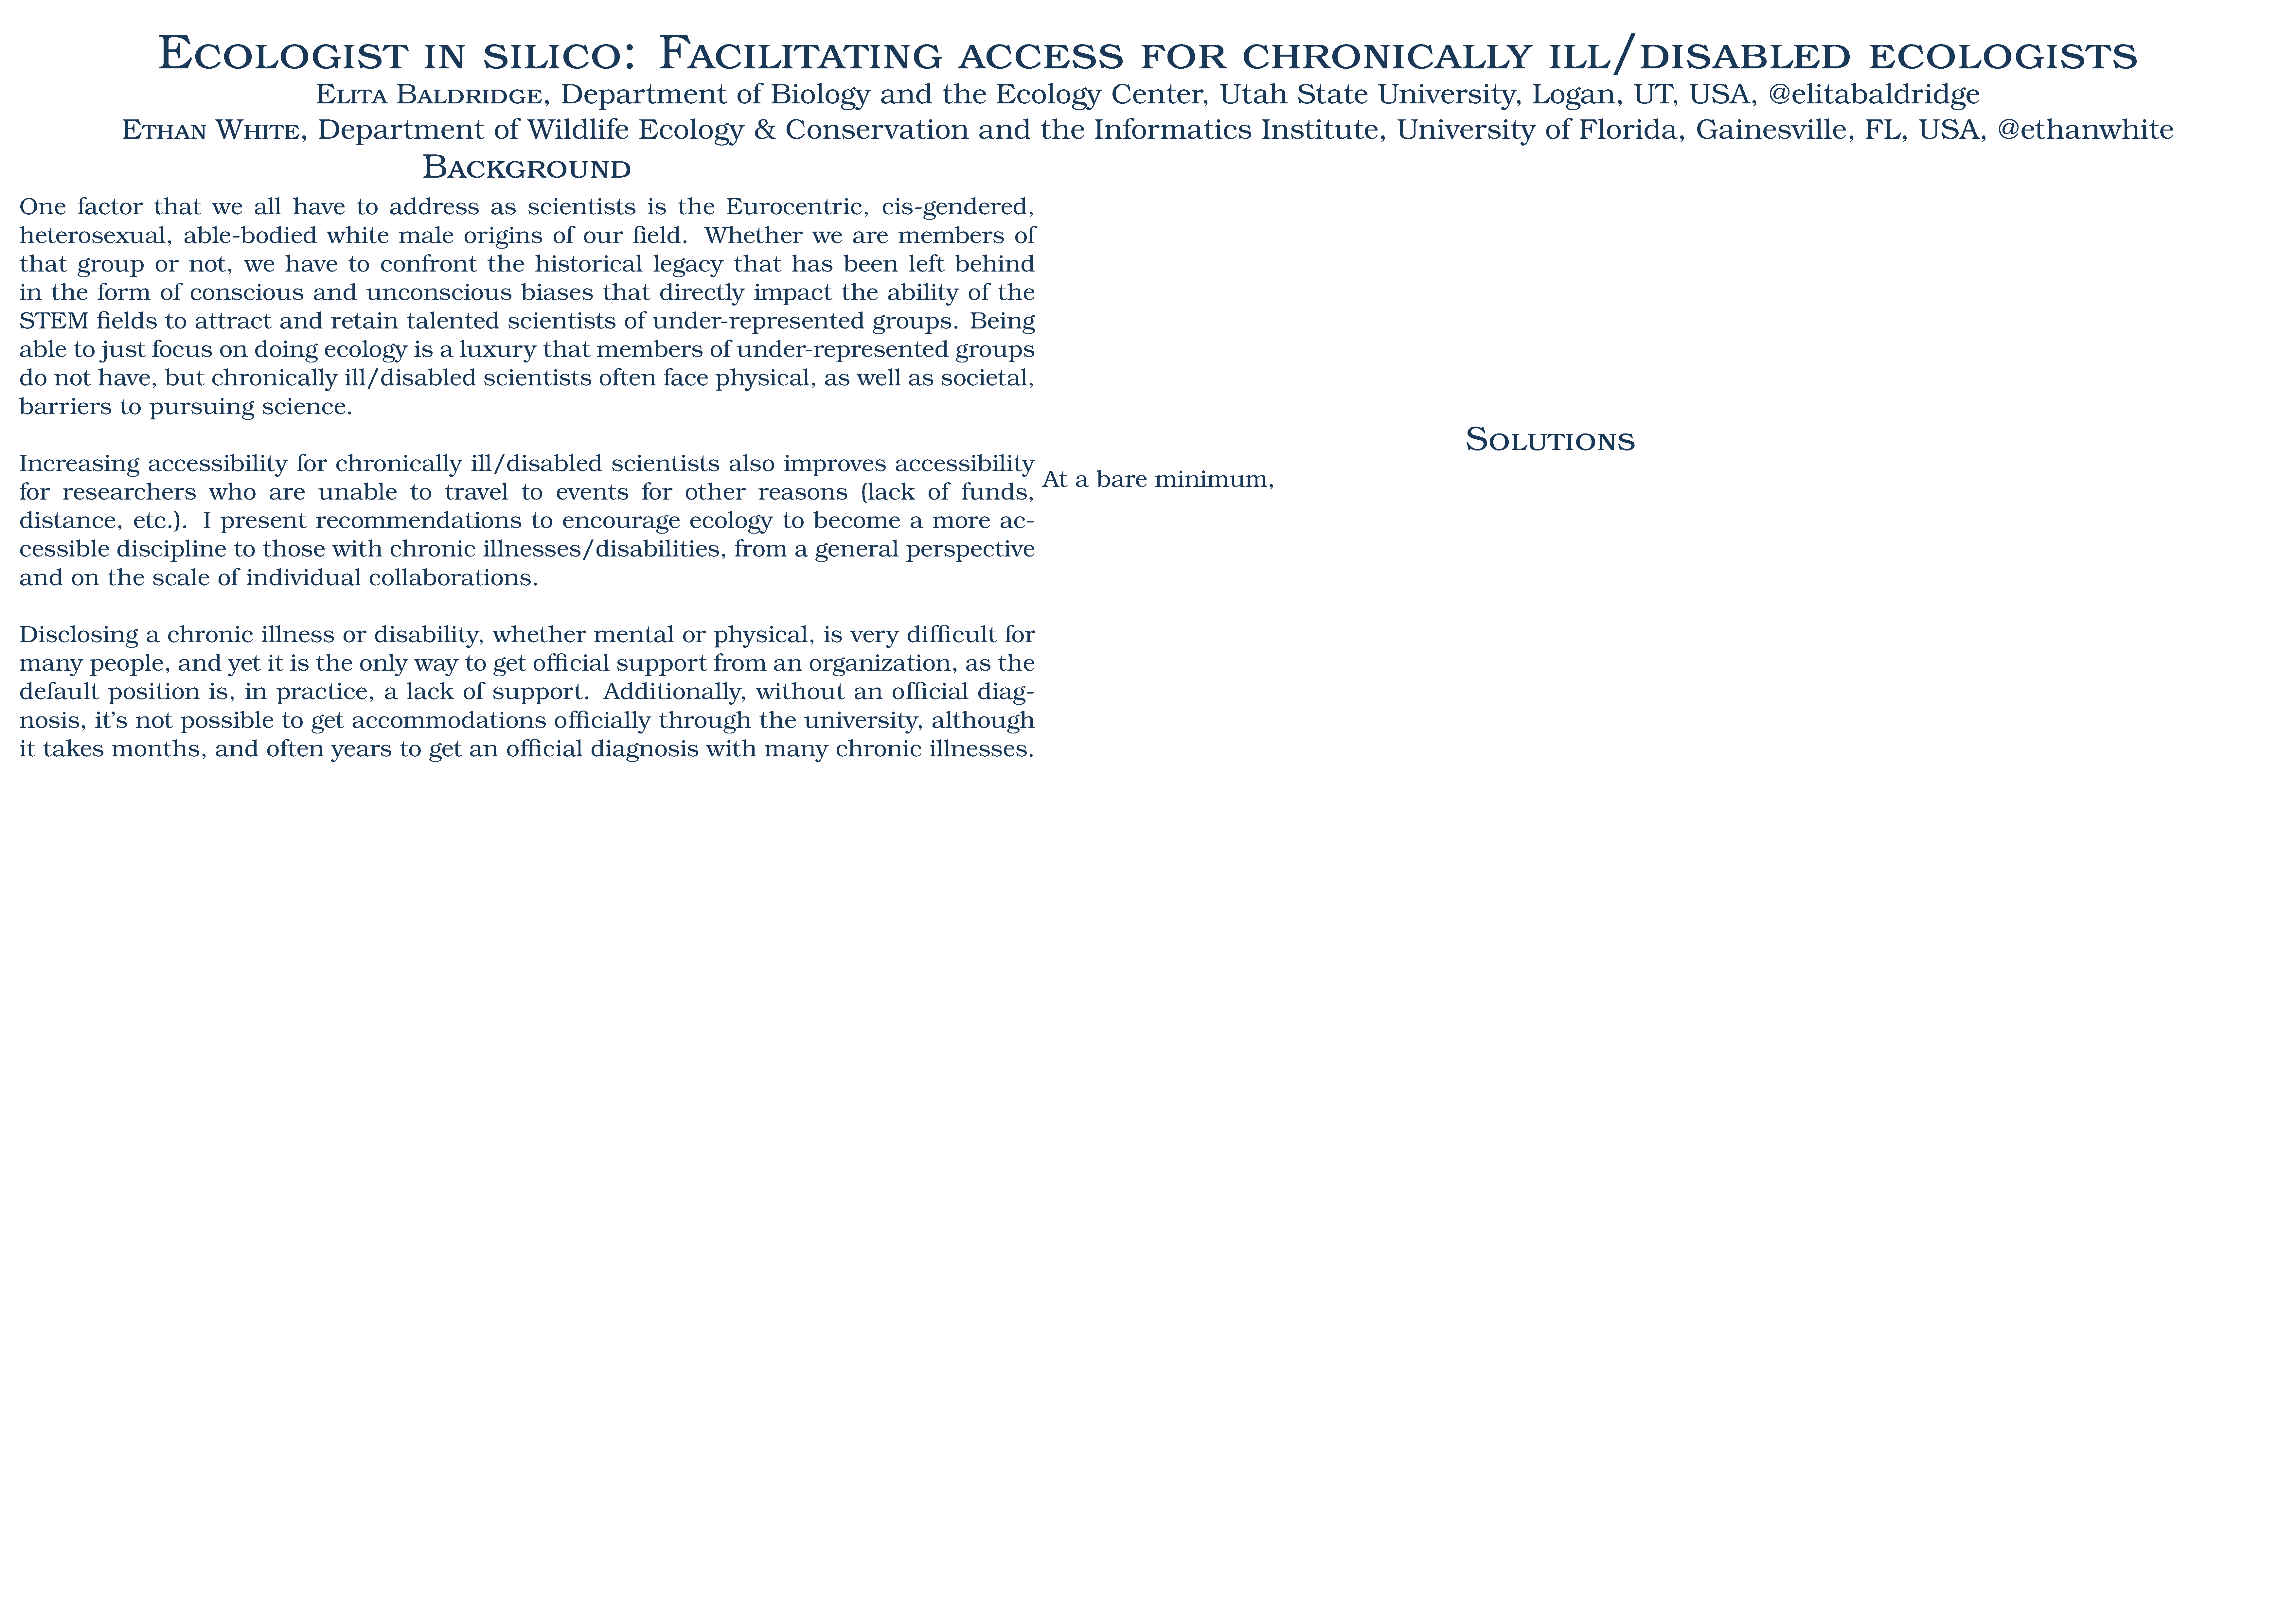
\includegraphics[scale=1]{../Pictures/Graphics/ESA_2015.png} 
\end{minipage}
~\\
~\\
\begin{center}
\includegraphics[scale=1]{../Pictures/Graphics/Weecology_use.png}
\end{center}
\end{minipage}
\hspace{1cm}
\begin{minipage}{0.25\linewidth}
\vspace{0.5cm}
~\\
\begin{Large}
\textsc{Inclusive Ecology}\\
\end{Large}
Self-advocacy takes up a lot of energy, and chronically ill/disabled researchers end up fighting the same battles repeatedly.  Having allies as part of an Inclusive Ecology section would help relieve some of the burden of self-advocacy faced by chronically-ill/disabled ecologists.\\
~\\
\textsc{Mission Statement}\\
To provide resources and support for all ecologists, regardless of race, sex, physical or mental ability or difference, gender identity or expression, sexual orientation, ethnicity, socio-economic status, culture or subculture, national origin,  parental status, politics, religion, or age.\\
~\\
~\\
\begin{minipage}{0.49\textwidth}
\textsc{Petition:}\\
~\\
\begin{minipage}{0.49\textwidth}
\includegraphics[scale=1]{../Pictures/Graphics/Inclusive_Ecology_petition.png}\\ 
\end{minipage}
\begin{minipage}{0.49\textwidth}
\url{https://goo.gl/8Hq3mr}\\
\end{minipage}
\end{minipage}
\begin{minipage}{0.49\textwidth}
\textsc{Proposed Bylaws:}\\
~\\
\begin{minipage}{0.49\textwidth}
\includegraphics[scale=1]{../Pictures/Graphics/Inclusive_Ecology_bylaws.png}\\
\end{minipage}
\begin{minipage}{0.49\textwidth} 
\url{https://goo.gl/Q6IMGO}\\
\end{minipage}
\end{minipage}
~\\
\begin{Large}
\textsc{Additional Reading/Resources}\\
\end{Large}
Conditionally Accepted blog:\\
\url{http://conditionallyaccepted.com/}\\
~\\
PhDisabled blog:\\
\url{http://phdisabled.wordpress.com/}\\
~\\
Color Blindness Simulator:\\
\url{http://www.color-blindness.com/coblis-color-blindness-simulator/}\\
~\\
Sighted Guide Technique:\\
\url{http://www.sightconnection.org/wp-content/uploads/sighted-guide.pdf}\\
~\\
Accessibility at Conferences:\\
\begin{minipage}{0.3\textwidth}
\includegraphics[scale=1]{../Pictures/Graphics/Access_storify.png}
\end{minipage}
\begin{minipage}{0.67\textwidth}
\url{https://goo.gl/nkS68f}\\
\end{minipage}
\\ 
\end{minipage}
\end{center}


\end{document}
